\section{Clases de la aplicación móvil}

\begin{figure}[H]
    \centering
    \makebox[\textwidth][c]{
        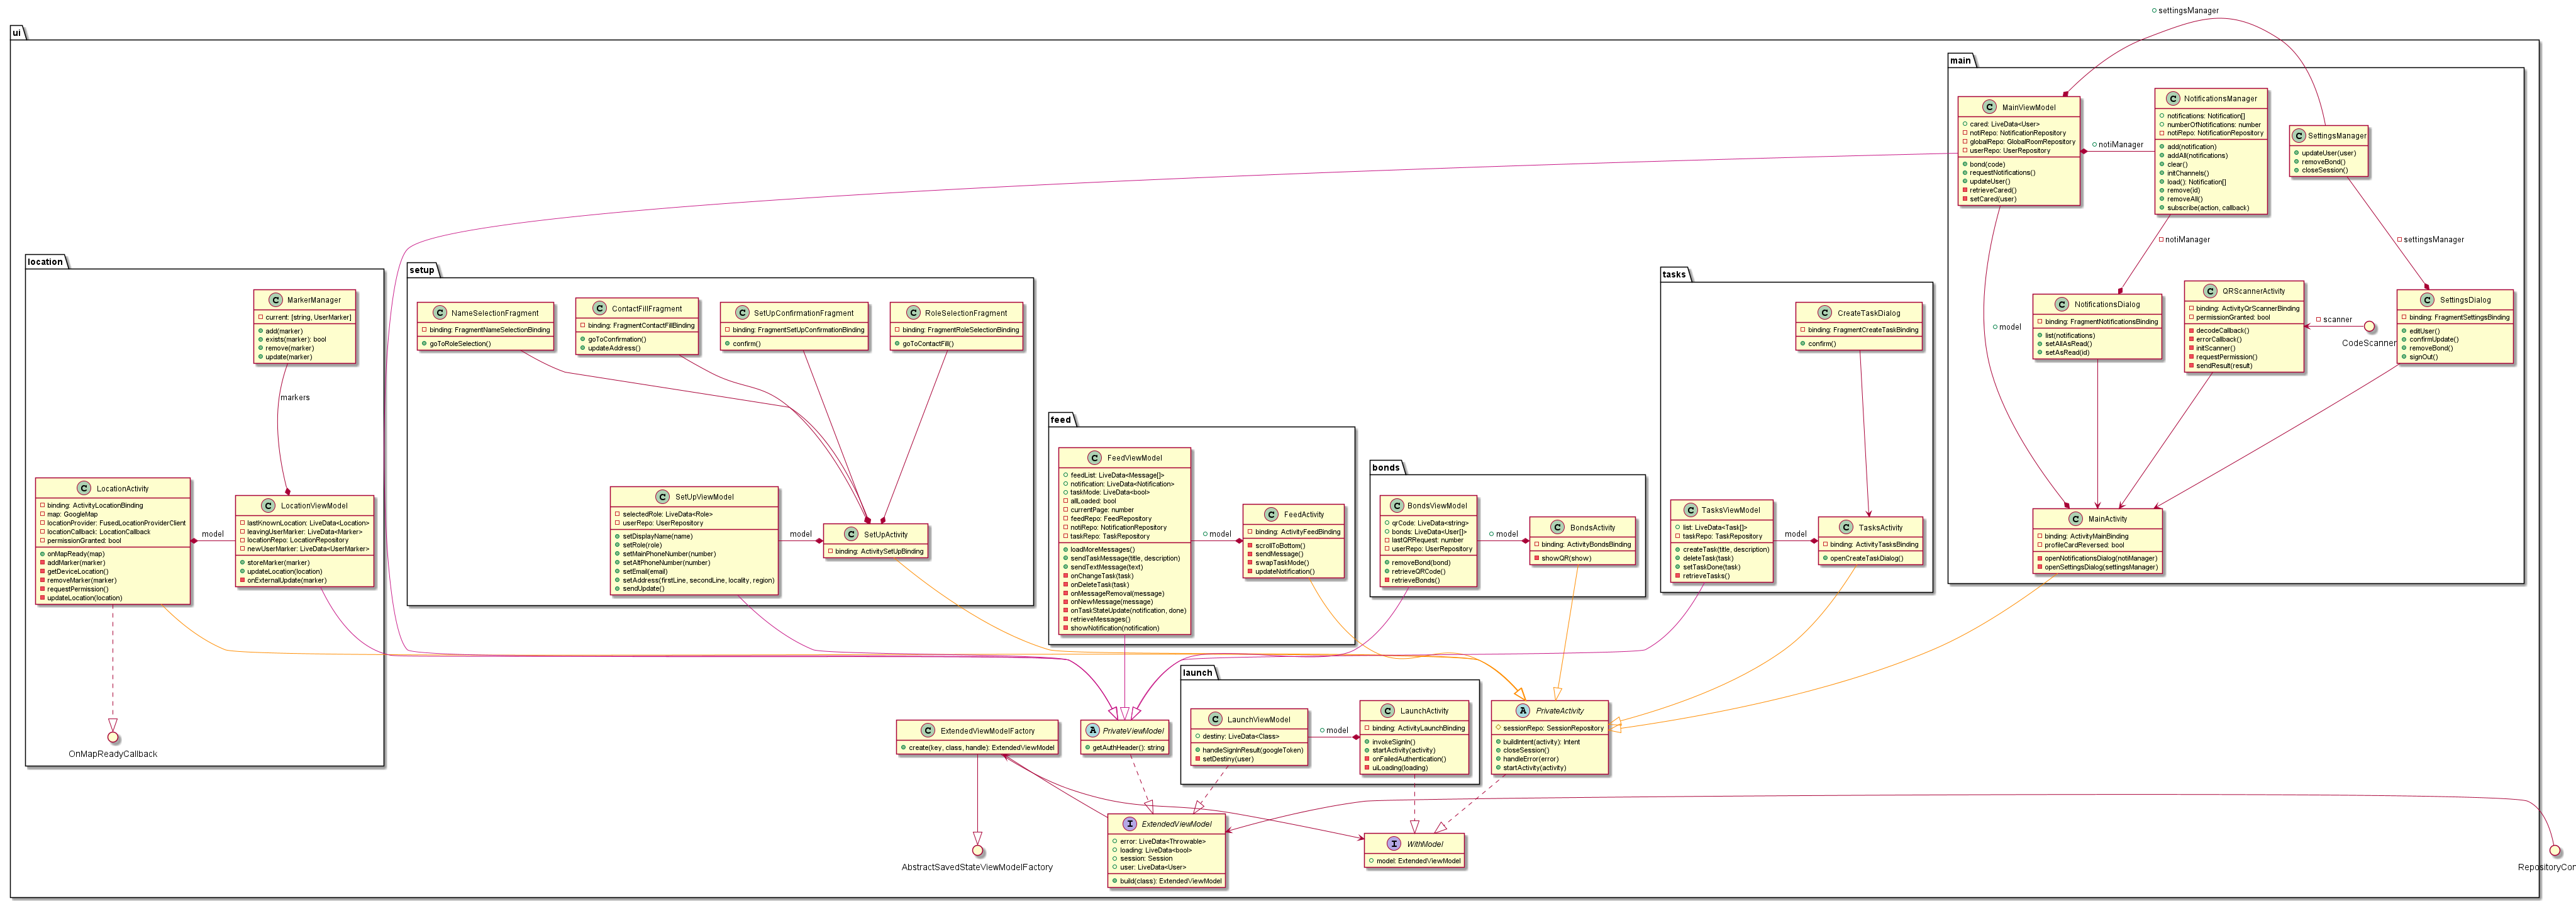
\includegraphics[width=1.3\textwidth]{images/Diseño/ClasesAppA.png}
    }
    \caption{Primera parte del diagrama de clases de la aplicación móvil}
    \label{fig:diagrama_clases_app_a}
\end{figure}

\begin{figure}[H]
    \centering
    \makebox[\textwidth][c]{
        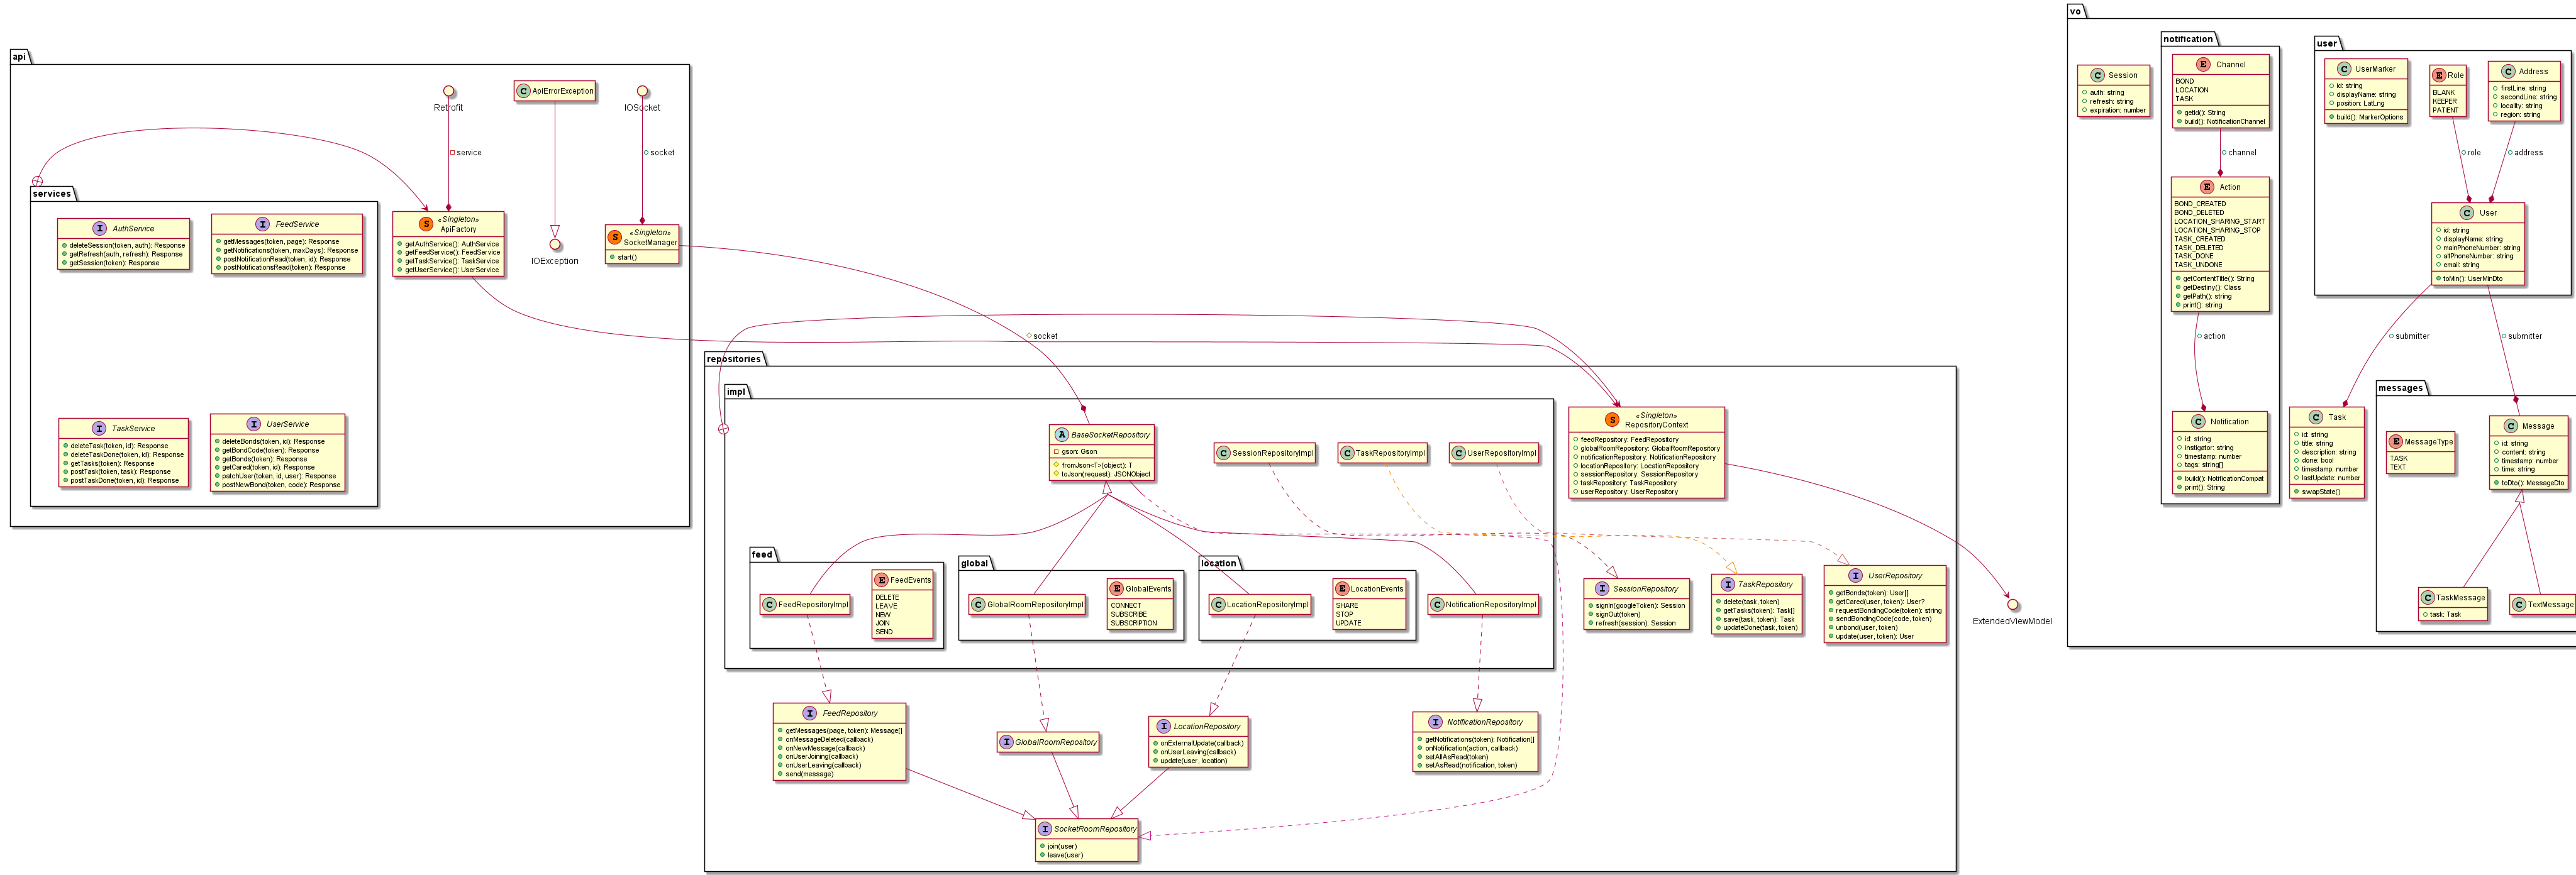
\includegraphics[width=1.3\textwidth]{images/Diseño/ClasesAppB.png}
    }
    \caption{Segunda parte del diagrama de clases de la aplicación móvil}
    \label{fig:diagrama_clases_app_b}
\end{figure}

\newpage
\subsection{UI}

\begin{longtable}{|p{0.25\textwidth} p{0.75\textwidth}|}
    \hline
    \multicolumn{2}{|l|}{\textbf{ExtendedViewModel}} \\ \hline \hline
    Descripción      & Interfaz común para los ViewModel a emplear en la aplicación \\ \hline
    \multicolumn{2}{|l|}{Propiedades} \\
    \emph{error}  & Contenedor del último error ocurrido  \\ 
    \emph{loading}  & Contenedor del estado de carga de la pantalla  \\ 
    \emph{session}  & Sesión actual \\ 
    \emph{user}  & Contenedor de los datos del usuario  \\ \hline
    \multicolumn{2}{|l|}{Funciones} \\
    \emph{build}  & Constructor para la creación en ExtendedViewModelFactory (\ref{dis:app:extended_viewmodel_factory})  \\ \hline
    \caption{Documentación de la interfaz ExtendedViewModel}
    \label{dis:app:extended_viewmodel}
\end{longtable}

\begin{longtable}{|p{0.25\textwidth} p{0.75\textwidth}|}
    \hline
    \multicolumn{2}{|l|}{\textbf{WithModel}} \\ \hline \hline
    Descripción      & Interfaz para clases que implementen un ExtendedViewModel (\ref{dis:app:extended_viewmodel}) \\ \hline
    \multicolumn{2}{|l|}{Propiedades} \\
    \emph{model}  & ExtendedViewModel implementado  \\ \hline
    \caption{Documentación de la interfaz WithModel}
    \label{dis:app:with_model}
\end{longtable}

\begin{longtable}{|p{0.25\textwidth} p{0.75\textwidth}|}
    \hline
    \multicolumn{2}{|l|}{\textbf{ExtendedViewModelFactory}} \\ \hline \hline
    Descripción      & Factoría de clases que implementan ExtendedViewModel (\ref{dis:app:extended_viewmodel}) \\ \hline
    \multicolumn{2}{|l|}{Funciones} \\
    \emph{create}  & Crea el ExtendedViewModel especificado  \\ \hline
    \caption{Documentación de la clase ExtendedViewModelFactory}
    \label{dis:app:extended_viewmodel_factory}
\end{longtable}

\begin{longtable}{|p{0.25\textwidth} p{0.75\textwidth}|}
    \hline
    \multicolumn{2}{|l|}{\textbf{PrivateViewModel}} \\ \hline \hline
    Descripción      & Implementación base de las clases ExtendedViewModel \\ \hline
    \multicolumn{2}{|l|}{Funciones} \\
    \emph{getAuthHeader}  & Obtiene y devuelve el encabezado de autenticación para las peticiones REST  \\ \hline
    \caption{Documentación de la clase PrivateViewModel}
    \label{dis:app:private_viewmodel}
\end{longtable}

\begin{longtable}{|p{0.25\textwidth} p{0.75\textwidth}|}
    \hline
    \multicolumn{2}{|l|}{\textbf{PrivateActivity}} \\ \hline \hline
    Descripción      & Implementación base de las actividades que implementen WithModel \\ \hline
    \multicolumn{2}{|l|}{Propiedades} \\
    \emph{sessionRepo}  & Repositorio para operaciones relacionadas con la sesión  \\ \hline
    \multicolumn{2}{|l|}{Funciones} \\
    \emph{buildIntent}  & Construye una intención de navegación a otra actividad con la información necesaria \\ 
    \emph{closeSession}  & Elimina los datos de sesión y retorna a LaunchActivity (\ref{dis:app:launch_activity}) \\
    \emph{handleError}  & Implementación por defecto para manejo de errores  \\ 
    \emph{startActivity}  & Inicia la actividad especificada  \\ \hline
    \caption{Documentación de la clase PrivateActivity}
    \label{dis:app:private_activity}
\end{longtable}

\vspace{-20pt}
\subsubsection{Launch}

\begin{longtable}{|p{0.3\textwidth} p{0.7\textwidth}|}
    \hline
    \multicolumn{2}{|l|}{\textbf{LaunchActivity}} \\ \hline \hline
    Descripción      & Actividad de inicio de la aplicación con el inicio de sesión \\ \hline
    \multicolumn{2}{|l|}{Propiedades} \\
    \emph{binding}  & Vista vinculada  \\
    \emph{model}  & Modelo de vista  \\ \hline
    \multicolumn{2}{|l|}{Funciones} \\
    \emph{invokeSign}  & Inicia el proceso de inicio de sesión  \\ 
    \emph{startActivity}  & Inicia la siguiente actividad  \\ 
    \emph{onFailedAuthentication}  & Gestiona errores de autenticación  \\ 
    \emph{uiLoading}  & Cambia el estado de carga de la interfaz  \\ \hline
    \caption{Documentación de la clase LaunchActivity}
    \label{dis:app:launch_activity}
\end{longtable}

\begin{longtable}{|p{0.25\textwidth} p{0.75\textwidth}|}
    \hline
    \multicolumn{2}{|l|}{\textbf{LaunchViewModel}} \\ \hline \hline
    Descripción      & Modelo de la vista de LaunchActivity \\ \hline
    \multicolumn{2}{|l|}{Propiedades} \\
    \emph{destiny}  & Contenedor para la siguiente actividad a la que navegar  \\ \hline
    \multicolumn{2}{|l|}{Funciones} \\
    \emph{handleSignInResult}  & Gestiona el resultado del intento de inicio de sesión con Google  \\
    \emph{setDestiny}  & Modifica el destino de navegación  \\ \hline
    \caption{Documentación de la clase LaunchViewModel}
    \label{dis:app:launch_viewmodel}
\end{longtable}

\subsubsection{Set up}

\begin{longtable}{|p{0.25\textwidth} p{0.75\textwidth}|}
    \hline
    \multicolumn{2}{|l|}{\textbf{SetUpActivity}} \\ \hline \hline
    Descripción      & Actividad de configuración de la cuenta de usuario en la creación de esta \\ \hline
    \multicolumn{2}{|l|}{Propiedades} \\
    \emph{binding}  & Vista vinculada  \\
    \emph{model}  & Modelo de vista  \\ \hline
    \caption{Documentación de la clase SetUpActivity}
    \label{dis:app:setup_activity}
\end{longtable}

\begin{longtable}{|p{0.3\textwidth} p{0.7\textwidth}|}
    \hline
    \multicolumn{2}{|l|}{\textbf{SetUpViewModel}} \\ \hline \hline
    Descripción      & Modelo de la vista de SetUpActivity \\ \hline
    \multicolumn{2}{|l|}{Propiedades} \\
    \emph{selectedRole}  & Contenedor del rol seleccionado  \\
    \emph{userRepo}  & Repositorio para gestionar los datos de usuario  \\ \hline
    \multicolumn{2}{|l|}{Funciones} \\
    \emph{setDisplayName}  & Establece el nombre  \\
    \emph{setRole}  & Establece el rol  \\
    \emph{setMainPhoneNumber}  & Establece el teléfono principal  \\
    \emph{setAltPhoneNumber}  & Establece el teléfono secundario  \\
    \emph{setEmail}  & Establece el email  \\
    \emph{setAddress}  & Establece la dirección postal  \\
    \emph{sendUpdate}  & Envía los datos del usuario para confirmarlo  \\ \hline
    \caption{Documentación de la clase SetUpViewModel}
    \label{dis:app:setup_viewmodel}
\end{longtable}

\begin{longtable}{|p{0.25\textwidth} p{0.75\textwidth}|}
    \hline
    \multicolumn{2}{|l|}{\textbf{NameSelectionFragment}} \\ \hline \hline
    Descripción      & Fragmento de selección del nombre del usuario \\ \hline
    \multicolumn{2}{|l|}{Propiedades} \\
    \emph{binding}  & Vista vinculada  \\ \hline
    \multicolumn{2}{|l|}{Funciones} \\
    \emph{goToRoleSelection}  & Navega a RoleSelectionFragment (\ref{dis:app:role_selection_fragment}) \\ \hline
    \caption{Documentación de la clase NameSelectionFragment}
    \label{dis:app:name_selection_fragment}
\end{longtable}

\hspace{\textwidth}

\begin{longtable}{|p{0.25\textwidth} p{0.75\textwidth}|}
    \hline
    \multicolumn{2}{|l|}{\textbf{RoleSelectionFragment}} \\ \hline \hline
    Descripción      & Fragmento de selección del rol del usuario \\ \hline
    \multicolumn{2}{|l|}{Propiedades} \\
    \emph{binding}  & Vista vinculada  \\ \hline
    \multicolumn{2}{|l|}{Funciones} \\
    \emph{goToContactFill}  & Navega a ContactFillFragment (\ref{dis:app:contact_fill_fragment}) \\ \hline
    \caption{Documentación de la clase RoleSelectionFragment}
    \label{dis:app:role_selection_fragment}
\end{longtable}

\vspace{-20pt}
\begin{longtable}{|p{0.25\textwidth} p{0.75\textwidth}|}
    \hline
    \multicolumn{2}{|l|}{\textbf{ContactFillFragment}} \\ \hline \hline
    Descripción      & Fragmento de especificación de datos de contacto del usuario \\ \hline
    \multicolumn{2}{|l|}{Propiedades} \\
    \emph{binding}  & Vista vinculada  \\ \hline
    \multicolumn{2}{|l|}{Funciones} \\
    \emph{goToConfirmation}  & Navega a SetUpConfirmationFragment (\ref{dis:app:setup_confirmation_fragment}) \\
    \emph{updateAddress}  & Actualiza la dirección del usuario  \\ \hline
    \caption{Documentación de la clase ContactFillFragment}
    \label{dis:app:contact_fill_fragment}
\end{longtable}

\vspace{-20pt}
\begin{longtable}{|p{0.25\textwidth} p{0.75\textwidth}|}
    \hline
    \multicolumn{2}{|l|}{\textbf{SetUpConfirmationFragment}} \\ \hline \hline
    Descripción      & Fragmento de confirmación de los datos introducidos \\ \hline
    \multicolumn{2}{|l|}{Propiedades} \\
    \emph{binding}  & Vista vinculada  \\ \hline
    \multicolumn{2}{|l|}{Funciones} \\
    \emph{confirm}  & Envía la confirmación de datos  \\ \hline
    \caption{Documentación de la clase SetUpConfirmationFragment}
    \label{dis:app:setup_confirmation_fragment}
\end{longtable}

\vspace{-20pt}
\subsubsection{Main}

\begin{longtable}{|p{0.3\textwidth} p{0.7\textwidth}|}
    \hline
    \multicolumn{2}{|l|}{\textbf{MainActivity}} \\ \hline \hline
    Descripción      & Actividad principal de la aplicación \\ \hline
    \multicolumn{2}{|l|}{Propiedades} \\
    \emph{binding}  & Vista vinculada  \\
    \emph{model}  & Modelo vinculado  \\
    \emph{openNotificationsDialog}  & Despliega el NotificationsDialog (\ref{dis:app:notifications_dialog}) \\ 
    \emph{openSettingssDialog}  & Despliega el SettingsDialog (\ref{dis:app:settings_dialog}) \\ \hline
    \caption{Documentación de la clase MainActivity}
    \label{dis:app:main_activity}
\end{longtable}

\vspace{-20pt}
\begin{longtable}{|p{0.25\textwidth} p{0.75\textwidth}|}
    \hline
    \multicolumn{2}{|l|}{\textbf{MainViewModel}} \\ \hline \hline
    Descripción      & Modelo de la vista MainActivity \\ \hline
    \multicolumn{2}{|l|}{Propiedades} \\
    \emph{cared}  & Contenedor de la información del paciente vinculado  \\
    \emph{notiManager}  & Gestor de notificaciones  \\
    \emph{notiRepo}  & Repositorio para las operaciones de notificaciones  \\
    \emph{globalRepo}  & Repositorio para las operaciones de la habitación global  \\
    \emph{userRepo}  & Repositorio para las operaciones de datos del usuario  \\ \hline
    \multicolumn{2}{|l|}{Funciones} \\
    \emph{bond}  & Envía una petición para crear un vínculo con otro usuario \\
    \emph{requestNotifications}  & Recupera las notificaciones no leídas \\ 
    \emph{updateUser} & Actualiza la información del usuario \\
    \emph{retrieveCared}  & Recupera la información del paciente vinculado \\ 
    \emph{setCared}  & Establece la información del paciente vinculado \\ \hline
    \caption{Documentación de la clase MainViewModel}
    \label{dis:app:main_view_model}
\end{longtable}

\vspace{-31pt}
\begin{longtable}{|p{0.25\textwidth} p{0.75\textwidth}|}
    \hline
    \multicolumn{2}{|l|}{\textbf{NotificationsDialog}} \\ \hline \hline
    Descripción      & Diálogo de gestión de las notificaciones \\ \hline
    \multicolumn{2}{|l|}{Propiedades} \\
    \emph{binding}  & Vista vinculada  \\
    \emph{cared}  & Información del paciente vinculado  \\
    \emph{notiManager}  & Gestor de notificaciones  \\ \hline
    \multicolumn{2}{|l|}{Funciones} \\
    \emph{list}  & Lista las notificaciones no leídas \\
    \emph{setAllAsRead}  & Marca todas las notificaciones como leídas \\ 
    \emph{setAsRead}  & Marca una notificación como leída \\ \hline
    \caption{Documentación de la clase NotificationsDialog}
    \label{dis:app:notifications_dialog}
\end{longtable}

\vspace{-31pt}
\begin{longtable}{|p{0.25\textwidth} p{0.75\textwidth}|}
    \hline
    \multicolumn{2}{|l|}{\textbf{SettingsDialog}} \\ \hline \hline
    Descripción      & Diálogo de gestión de las notificaciones \\ \hline
    \multicolumn{2}{|l|}{Propiedades} \\
    \emph{binding}  & Vista vinculada  \\ \hline
    \multicolumn{2}{|l|}{Funciones} \\
    \emph{editUser} & Abre la opción de edición del usuario \\
    \emph{cconfirmUpdate} & Confirma la actualización de datos del usuario \\
    \emph{removeBond} & Elimina el vínculo \\
    \emph{signOut}  & Invoca el cierre de sesión \\ \hline
    \caption{Documentación de la clase SettingsDialog}
    \label{dis:app:settings_dialog}
\end{longtable}

\begin{longtable}{|p{0.35\textwidth} p{0.65\textwidth}|}
    \hline
    \multicolumn{2}{|l|}{\textbf{NotificationsManager}} \\ \hline \hline
    Descripción      & Gestor de las notificaciones \\ \hline
    \multicolumn{2}{|l|}{Propiedades} \\
    \emph{notifications}  & Lista de notificaciones no leídas  \\
    \emph{numberOfNotifications}  & Número de notificaciones no leídas  \\
    \emph{notiRepo}  & Repositorio para las operaciones de notificaciones  \\ \hline
    \multicolumn{2}{|l|}{Funciones} \\
    \emph{add}  & Añade una notificación a la lista \\
    \emph{addAll}  & Añade un conjunto de notificaciones a la lista \\ 
    \emph{clear}  & Vacía la lista de notificaciones \\
    \emph{initChannels} & Inicia los canales de notificación \\
    \emph{load}  & Carga las notificaciones no leídas \\
    \emph{remove}  & Sustrae una notificación de la lista \\ 
    \emph{removeAll}  & Sustrae un conjunto de notificaciones de la lista \\
    \emph{subscribe}  & Subscribe el WebSocket a los eventos de notificaciones \\  \hline
    \caption{Documentación de la clase NotificationsManager}
    \label{dis:app:notifications_manager}
\end{longtable}

\vspace{-25pt}
\begin{longtable}{|p{0.25\textwidth} p{0.75\textwidth}|}
    \hline
    \multicolumn{2}{|l|}{\textbf{SettingsManager}} \\ \hline \hline
    Descripción      & Gestor de las opciones \\ \hline
    \multicolumn{2}{|l|}{Funciones} \\
    \emph{updateUser} & Actualiza los datos del usuario con los nuevos \\
    \emph{removeBond} & Elimina el vínculo \\
    \emph{closeSession}  & Cierra la sesión actual \\  \hline
    \caption{Documentación de la clase SettingsManager}
    \label{dis:app:settings_manager}
\end{longtable}

\vspace{-25pt}
\begin{longtable}{|p{0.25\textwidth} p{0.75\textwidth}|}
    \hline
    \multicolumn{2}{|l|}{\textbf{QRScannerActivity}} \\ \hline \hline
    Descripción      & Escáner para la lectura del código QR \\ \hline
    \multicolumn{2}{|l|}{Propiedades} \\
    \emph{binding}  & Vista vinculada  \\
    \emph{permissionGranted}  & Estado de los permisos para el uso de la cámara  \\ \hline
    \multicolumn{2}{|l|}{Funciones} \\
    \emph{decodeCallback}  & Maneja el resultado de la descodificación \\
    \emph{errorCallback}  & Gestiona errores en la lectura \\ 
    \emph{initScanner}  & Inicializa el escáner \\
    \emph{requestPermission}  & Solicita el permiso del usuario para usar la cámara \\ 
    \emph{sendResult}  & Envía el resultado de la lectura a la actividad invocada \\ \hline
    \caption{Documentación de la clase QRScannerActivity}
    \label{dis:app:qr_scanner_activity}
\end{longtable}

\subsubsection{Bonds}

\begin{longtable}{|p{0.25\textwidth} p{0.75\textwidth}|}
    \hline
    \multicolumn{2}{|l|}{\textbf{BondsActivity}} \\ \hline \hline
    Descripción      & Actividad para la gestión de los vínculos \\ \hline
    \multicolumn{2}{|l|}{Propiedades} \\
    \emph{binding}  & Vista vinculada  \\
    \emph{model}  & Modelo de vista  \\ \hline
    \multicolumn{2}{|l|}{Funciones} \\
    \emph{showQr}  & Muestra un QR de vinculación \\ \hline
    \caption{Documentación de la clase BondsActivity}
    \label{dis:app:bonds_activity}
\end{longtable}

\vspace{-25pt}
\begin{longtable}{|p{0.25\textwidth} p{0.75\textwidth}|}
    \hline
    \multicolumn{2}{|l|}{\textbf{BondsViewModel}} \\ \hline \hline
    Descripción      & Modelo de la vista BondsActivity \\ \hline
    \multicolumn{2}{|l|}{Propiedades} \\
    \emph{bonds}  & Lista de usuarios vinculados \\
    \emph{lastQRRequest}  & Instante de la última petición de código QR  \\ 
    \emph{qrCode}  & Código QR para mostrar  \\
    \emph{userRepo}  & Repositorio para las operaciones de datos del usuario  \\ \hline
    \multicolumn{2}{|l|}{Funciones} \\
    \emph{removeBond} & Elimina el vínculo \\
    \emph{retrieveBonds}  & Recupera la información de los usuarios asociados \\
    \emph{retrieveQRCode}  & Solicita un código QR para vinculación \\ \hline
    \caption{Documentación de la clase BondsViewModel}
    \label{dis:app:bonds_view_model}
\end{longtable}

\vspace{-30pt}
\subsubsection{Feed}

\begin{longtable}{|p{0.25\textwidth} p{0.75\textwidth}|}
    \hline
    \multicolumn{2}{|l|}{\textbf{FeedActivity}} \\ \hline \hline
    Descripción      & Actividad de la aplicación con el chat entre usuarios asociados \\ \hline
    \multicolumn{2}{|l|}{Propiedades} \\
    \emph{binding}  & Vista vinculada  \\
    \emph{model}  & Modelo de vista  \\ \hline
    \multicolumn{2}{|l|}{Funciones} \\
    \emph{scrollToBottom}  & Mueve el feed hasta el final \\
    \emph{sendMessage}  & Envía un mensaje  \\ 
    \emph{swapTaskMode}  & Cambia al modo de envío de tareas  \\ 
    \emph{updateNotification}  & Actualiza la notificación en pantalla  \\  \hline
    \caption{Documentación de la clase FeedActivity}
    \label{dis:app:feed_activity}
\end{longtable}

\begin{longtable}{|p{0.25\textwidth} p{0.75\textwidth}|}
    \hline
    \multicolumn{2}{|l|}{\textbf{FeedViewModel}} \\ \hline \hline
    Descripción      & Modelo de la vista FeedActivity \\ \hline
    \multicolumn{2}{|l|}{Propiedades} \\
    \emph{allLoaded}  & Bandera de indicación de que todos los mensajes fueron cargados  \\
    \emph{currentPage}  & Última página de mensajes cargada  \\
    \emph{feedList}  & Contenedor de los mensajes cargados  \\
    \emph{feedRepo}  & Repositorio para las operaciones del feed  \\
    \emph{notification}  & Contenedor de la última notificación a mostrar  \\
    \emph{notiRepo}  & Repositorio para las operaciones de notificaciones  \\
    \emph{taskMode}  & Contenedor del estado del modo de creación de tareas  \\
    \emph{taskRepo}  & Repositorio para las operaciones de las tareas  \\ \hline
    \multicolumn{2}{|l|}{Funciones} \\
    \emph{loadMoreMessages}  & Carga una nueva páginas de mensajes \\
    \emph{onChangeTask}  & Maneja la modificación de una tarea  \\ 
    \emph{onDeleteTask}  & Maneja la eliminación de una tarea  \\ 
    \emph{onMessageRemoval}  & Maneja la eliminación de un mensaje  \\ 
    \emph{onNewMessage}  & Maneja la entrada de nuevos mensajes  \\ 
    \emph{onTaskStateUpdate}  & Maneja el cambio de estado de una tarea  \\ 
    \emph{retrieveMessages}  & Recupera los mensajes  \\ 
    \emph{sendTaskMessage}  & Envía una tarea  \\ 
    \emph{sendTextMessage}  & Envía un mensaje de texto  \\
    \emph{showNotification}  & Muestra una notificación  \\  \hline
    \caption{Documentación de la clase FeedViewModel}
    \label{dis:app:feed_view_model}
\end{longtable}

\newpage
\subsubsection{Location}

\begin{longtable}{|p{0.25\textwidth} p{0.75\textwidth}|}
    \hline
    \multicolumn{2}{|l|}{\textbf{LocationActivity}} \\ \hline \hline
    Descripción      & Actividad con el mapa de la geolocalización \\ \hline
    \multicolumn{2}{|l|}{Propiedades} \\
    \emph{binding}  & Vista vinculada  \\
    \emph{map}  & Mapa de Google  \\
    \emph{locationProvider}  & Cliente proveedor de la localización del usuario  \\
    \emph{locationCallback}  & Llamada para actualizaciones de la localización \\
    \emph{permissionGranted}  & Estado de los permisos de localización \\
    \emph{modelo}  & Modelo de vista  \\ \hline
    \multicolumn{2}{|l|}{Funciones} \\
    \emph{addMarker}  & Añade un nuevo marcador al mapa  \\
    \emph{getDeviceLocation}  & Recupera la localización del usuario \\ 
    \emph{onMapReady}  & Gestiona la carga del mapa  \\
    \emph{removeMarker}  & Elimina un marcador \\
    \emph{requestPermission}  & Solicita el permiso del usuario para usar la geolocalización  \\
    \emph{updateLocation}  & Actualiza un marcador  \\  \hline
    \caption{Documentación de la clase LocationActivity}
    \label{dis:app:location_activity}
\end{longtable}

\begin{longtable}{|p{0.25\textwidth} p{0.75\textwidth}|}
    \hline
    \multicolumn{2}{|l|}{\textbf{LocationViewModel}} \\ \hline \hline
    Descripción      & Modelo de la vista LocationActivity \\ \hline
    \multicolumn{2}{|l|}{Propiedades} \\
    \emph{markers}  & Gestor de marcadores  \\
    \emph{leavingUser}  & Contenedor de un marcador a eliminar  \\
    \emph{locationRepo}  & Repositorio para operaciones relacionadas con la localización  \\
    \emph{newUserMarker}  & Contenedor de un nuevo marcador  \\\hline
    \multicolumn{2}{|l|}{Funciones} \\
    \emph{onExternalUpdate}  & Gestiona una actualización de ubicación de terceros \\ 
    \emph{storeMarker}  & Almacena un nuevo marcador \\
    \emph{updateLocation}  & Envía la localización al resto de usuarios \\\hline
    \caption{Documentación de la clase LocationViewModel}
    \label{dis:app:location_viewmodel}
\end{longtable}

\newpage
\begin{longtable}{|p{0.25\textwidth} p{0.75\textwidth}|}
    \hline
    \multicolumn{2}{|l|}{\textbf{MarkerManager}} \\ \hline \hline
    Descripción      & Gestiona los marcadores de usuario a mostrar en el mapa \\ \hline
    \multicolumn{2}{|l|}{Propiedades} \\
    \emph{current}  & Mapa actual de usuarios y marcadores a mostrar  \\\hline
    \multicolumn{2}{|l|}{Funciones} \\
    \emph{add}  & Añade un nuevo marcador \\ 
    \emph{exists}  & Comprueba si existe un marcador \\
    \emph{remove}  & Elimina un marcador \\
    \emph{update}  & Actualiza un marcador \\ \hline
    \caption{Documentación de la clase MarkerManager}
    \label{dis:app:marker_manager}
\end{longtable}

\subsubsection{Tasks}

\begin{longtable}{|p{0.25\textwidth} p{0.75\textwidth}|}
    \hline
    \multicolumn{2}{|l|}{\textbf{TasksActivity}} \\ \hline \hline
    Descripción      & Actividad para la gestión de tareas \\ \hline
    \multicolumn{2}{|l|}{Propiedades} \\
    \emph{binding}  & Vista vinculada  \\
    \emph{model}  & Modelo de vista  \\ \hline
    \multicolumn{2}{|l|}{Funciones} \\
    \emph{openCreateTask}  & Despliega CreateTaskDialog (\ref{dis:app:create_task_dialog})  \\ \hline
    \caption{Documentación de la clase TasksActivity}
    \label{dis:app:tasks_activity}
\end{longtable}

\begin{longtable}{|p{0.25\textwidth} p{0.75\textwidth}|}
    \hline
    \multicolumn{2}{|l|}{\textbf{TasksViewModel}} \\ \hline \hline
    Descripción      & Modelo de la vista TasksActivity \\ \hline
    \multicolumn{2}{|l|}{Propiedades} \\
    \emph{list}  & Lista de tareas relevantes del usuario  \\
    \emph{taskRepo}  & Repositorio para las operaciones con las tareas  \\ \hline
    \multicolumn{2}{|l|}{Funciones} \\
    \emph{createTask}  & Envía una nueva tarea para crear \\
    \emph{deleteTask}  & Envía una petición para eliminar una tarea \\
    \emph{setTaskDone}  & Cambia el estado de una tarea \\
    \emph{retrieveTasks}  & Recupera la lista de tareas relevantes del usuario \\ \hline
    \caption{Documentación de la clase TasksViewModel}
    \label{dis:app:tasks_view_model}
\end{longtable}

\begin{longtable}{|p{0.25\textwidth} p{0.75\textwidth}|}
    \hline
    \multicolumn{2}{|l|}{\textbf{CreateTaskDialog}} \\ \hline \hline
    Descripción      & Actividad para la gestión de tareas \\ \hline
    \multicolumn{2}{|l|}{Propiedades} \\
    \emph{binding}  & Vista vinculada  \\ \hline
    \multicolumn{2}{|l|}{Funciones} \\
    \emph{confirm}  & Confirma la tarea creada  \\ \hline
    \caption{Documentación de la clase CreateTaskDialog}
    \label{dis:app:create_task_dialog}
\end{longtable}

\vspace{-30pt}
\subsection{Repositories}

\vspace{-10pt}
\begin{longtable}{|p{0.3\textwidth} p{0.7\textwidth}|}
    \hline
    \multicolumn{2}{|l|}{\textbf{RepositoryContext}} \\ \hline \hline
    Descripción      & Inyector de repositorios para los modelos de vista \\ \hline
    \multicolumn{2}{|l|}{Propiedades} \\
    \emph{feedRepository}  & Proporciona un FeedRepository (\ref{dis:app:feed_repository}) \\
    \emph{globalRoomRepository}  & Proporciona un GlobalRoomRepository (\ref{dis:app:global_room_repository})  \\
    \emph{notificationRepository}  & Proporciona un NotificationRepository (\ref{dis:app:notification_repository})  \\
    \emph{locationRepository}  & Proporciona un LocationRepository (\ref{dis:app:location_repository})  \\
    \emph{sessionRepository}  & Proporciona un SessionRepository (\ref{dis:app:session_repository})  \\
    \emph{taskRepository}  & Proporciona un TaskRepository (\ref{dis:app:tasks_repository})  \\
    \emph{userRepository}  & Proporciona un UserRepository (\ref{dis:app:user_repository})  \\ \hline
    \caption{Documentación de la entidad RepositoryContext}
    \label{dis:app:repository_context}
\end{longtable}

\vspace{-20pt}
\begin{longtable}{|p{0.25\textwidth} p{0.75\textwidth}|}
    \hline
    \multicolumn{2}{|l|}{\textbf{SocketRoomRepository}} \\ \hline \hline
    Descripción      & Interfaz de repositorios con lógica WebSocket \\ \hline
    \multicolumn{2}{|l|}{Funciones} \\
    \emph{join}  & Gestiona la unión a una sala  \\ 
    \emph{leave}  & Gestione el abandono de una sala  \\ \hline
    \caption{Documentación de la interfaz SocketRoomRepository}
    \label{dis:app:socket_room_repository}
\end{longtable}

\vspace{-20pt}
\begin{longtable}{|p{0.25\textwidth} p{0.75\textwidth}|}
    \hline
    \multicolumn{2}{|l|}{\textbf{BaseSocketRepository}} \\ \hline \hline
    Descripción      & Implementación base para los repositorios con WebSockets \\ \hline
    \multicolumn{2}{|l|}{Propiedades} \\
    \emph{gson}  & Conversor entre objetos JSON y instancias del código \\ \hline
    \multicolumn{2}{|l|}{Funciones} \\
    \emph{fromJson}  & Instancia un objeto generado a partir de un JSON  \\ 
    \emph{toJson}  & Transforma un objeto en un JSON  \\ \hline
    \caption{Documentación de la clase BaseSocketRepository}
    \label{dis:app:base_socket_repository}
\end{longtable}

\subsubsection{FeedRepository}

\begin{longtable}{|p{0.25\textwidth} p{0.75\textwidth}|}
    \hline
    \multicolumn{2}{|l|}{\textbf{FeedRepository}} \\ \hline \hline
    Descripción      & Interfaz para la gestión de las operaciones relacionadas con el feed \\ \hline
    \multicolumn{2}{|l|}{Funciones} \\
    \emph{getMessages}  & Recupera la lista de mensajes \\
    \emph{onMessageDeleted}  & Suscribe una acción a la eliminación de un mensaje \\
    \emph{onNewMessage}  & Suscribe una acción a la entrada de un nuevo mensaje \\
    \emph{onUserJoining}  & Suscribe una acción a la conexión de un usuario a la sala del feed \\
    \emph{onUserLeaving}  & Suscribe una acción a la desconexión de un usuario a la sala del feed \\
    \emph{send}  & Envía un mensaje \\ \hline
    \caption{Documentación de la interfaz FeedRepository}
    \label{dis:app:feed_repository}
\end{longtable}

\begin{figure}[H]
\begin{longtable}{|p{0.25\textwidth} p{0.75\textwidth}|}
    \hline
    \multicolumn{2}{|l|}{\textbf{FeedRepositoryImpl}} \\ \hline \hline
    Descripción      & Implementación de la interfaz FeedRepository \\ \hline
    \caption{Documentación de la implementación de FeedRepository}
    \label{dis:app:feed_repository_impl}
\end{longtable}
\end{figure}

\begin{longtable}{|p{0.25\textwidth} p{0.75\textwidth}|}
    \hline
    \multicolumn{2}{|l|}{\textbf{FeedEvent}} \\ \hline \hline
    Descripción      & Eventos de la sala del feed \\ \hline
    \multicolumn{2}{|l|}{Valores} \\
    \emph{DELETE}  & Eliminación de un mensaje  \\
    \emph{LEAVE}  & Abandono de la sala  \\
    \emph{NEW}  & Nuevo usuario en la sala  \\
    \emph{JOIN}  & Unión a la sala  \\
    \emph{SEND}  & Envío de un nuevo mensaje  \\ \hline
    \caption{Documentación del enumerado FeedEvent de la aplicación}
    \label{dis:app:feed_event}
\end{longtable}

\subsubsection{GlobalRoomRepository}

\begin{longtable}{|p{0.25\textwidth} p{0.75\textwidth}|}
    \hline
    \multicolumn{2}{|l|}{\textbf{GlobalRoomRepository}} \\ \hline \hline
    Descripción      & Interfaz para la gestión de la conexión con la sala global \\ \hline
    \caption{Documentación de la interfaz GlobalRoomRepository}
    \label{dis:app:global_room_repository}
\end{longtable}

\begin{longtable}{|p{0.25\textwidth} p{0.75\textwidth}|}
    \hline
    \multicolumn{2}{|l|}{\textbf{GlobalRoomRepositoryImpl}} \\ \hline \hline
    Descripción      & Implementación de la interfaz GlobalRoomRepository \\ \hline
    \caption{Documentación de la implementación de GlobalRoomRepository}
    \label{dis:app:global_room_repository_impl}
\end{longtable}

\begin{longtable}{|p{0.25\textwidth} p{0.75\textwidth}|}
    \hline
    \multicolumn{2}{|l|}{\textbf{GlobalEvent}} \\ \hline \hline
    Descripción      & Eventos de la sala global \\ \hline
    \multicolumn{2}{|l|}{Valores} \\
    \emph{CONNECT}  & Conexión del WebSocket  \\
    \emph{SUBSCRIBE}  & Unión a la sala  \\
    \emph{SUBSCRIPTION} & Nuevo usuario en la sala  \\ \hline
    \caption{Documentación del enumerado GlobalEvent de la aplicación}
    \label{dis:app:global_event}
\end{longtable}

\subsubsection{LocationRepository}

\begin{longtable}{|p{0.25\textwidth} p{0.75\textwidth}|}
    \hline
    \multicolumn{2}{|l|}{\textbf{LocationRepository}} \\ \hline \hline
    Descripción      & Interfaz para operaciones relacionadas con la geolocalización \\ \hline
    \multicolumn{2}{|l|}{Funciones} \\
    \emph{onExternalUpdate}  & Suscribe una acción a la llegada de actualizaciones \\
    \emph{onUserLeaving}  & Suscribe una acción a la desconexión de un usuario de la sala \\
    \emph{update}  & Actualiza la localización del usuario \\ \hline
    \caption{Documentación de la interfaz LocationRepository}
    \label{dis:app:location_repository}
\end{longtable}

\begin{longtable}{|p{0.25\textwidth} p{0.75\textwidth}|}
    \hline
    \multicolumn{2}{|l|}{\textbf{LocationRepositoryImpl}} \\ \hline \hline
    Descripción      & Implementación de la interfaz LocationRepository \\ \hline
    \caption{Documentación de la implementación de LocationRepository}
    \label{dis:app:location_repository_impl}
\end{longtable}

\vspace{-20pt}
\begin{longtable}{|p{0.25\textwidth} p{0.75\textwidth}|}
    \hline
    \multicolumn{2}{|l|}{\textbf{LocationEvent}} \\ \hline \hline
    Descripción      & Eventos de la sala Location \\ \hline
    \multicolumn{2}{|l|}{Valores} \\
    \emph{SHARE}  & Unión a la sala  \\
    \emph{STOP} & Abandono de la sala  \\
    \emph{UPDATE} & Envío de una nueva ubicación  \\ \hline
    \caption{Documentación del enumerado LocationEvent de la aplicación}
    \label{dis:app:location_event}
\end{longtable}

\subsubsection{NotificationRepository}

\begin{longtable}{|p{0.25\textwidth} p{0.75\textwidth}|}
    \hline
    \multicolumn{2}{|l|}{\textbf{NotificationRepository}} \\ \hline \hline
    Descripción      & Interfaz para operaciones relacionadas con las notificaciones \\ \hline
    \multicolumn{2}{|l|}{Funciones} \\
    \emph{getNotifications}  & Recupera la lista de notificaciones \\
    \emph{onNotification}  & Suscribe una acción a la llegada de una nueva notificación \\
    \emph{setAllAsRead}  & Marca todas las notificaciones como leídas \\
    \emph{setAsRead}  & Marca una notificación como leída \\ \hline
    \caption{Documentación de la interfaz NotificationRepository}
    \label{dis:app:notification_repository}
\end{longtable}

\begin{longtable}{|p{0.25\textwidth} p{0.75\textwidth}|}
    \hline
    \multicolumn{2}{|l|}{\textbf{NotificationRepositoryImpl}} \\ \hline \hline
    Descripción      & Implementación de la interfaz NotificationRepository \\ \hline
    \caption{Documentación de la implementación de NotificationRepository}
    \label{dis:app:notification_repository_impl}
\end{longtable}

\subsubsection{SessionRepository}

\begin{longtable}{|p{0.25\textwidth} p{0.75\textwidth}|}
    \hline
    \multicolumn{2}{|l|}{\textbf{SessionRepository}} \\ \hline \hline
    Descripción      & Interfaz para operaciones relacionadas con la sesión \\ \hline
    \multicolumn{2}{|l|}{Funciones} \\
    \emph{signIn}   & Inicia la sesión del usuario \\
    \emph{signOut}  & Cierra la sesión del usuario \\
    \emph{refresh}  & Refresca la sesión del usuario \\ \hline
    \caption{Documentación de la interfaz SessionRepository}
    \label{dis:app:session_repository}
\end{longtable}

\begin{longtable}{|p{0.25\textwidth} p{0.75\textwidth}|}
    \hline
    \multicolumn{2}{|l|}{\textbf{SessionRepositoryImpl}} \\ \hline \hline
    Descripción      & Implementación de la interfaz SessionRepository \\ \hline
    \caption{Documentación de la implementación de SessionRepository}
    \label{dis:app:session_repository_impl}
\end{longtable}

\newpage
\subsubsection{TasksRepository}

\begin{longtable}{|p{0.25\textwidth} p{0.75\textwidth}|}
    \hline
    \multicolumn{2}{|l|}{\textbf{TasksRepository}} \\ \hline \hline
    Descripción      & Interfaz para operaciones relacionadas con las tareas \\ \hline
    \multicolumn{2}{|l|}{Funciones} \\
    \emph{delete}  & Elimina una tarea \\
    \emph{getTasks}  & Recupera las tareas \\
    \emph{save}  & Guarda una tarea \\
    \emph{update}  & Actualiza una tarea \\ \hline
    \caption{Documentación de la interfaz TasksRepository}
    \label{dis:app:tasks_repository}
\end{longtable}

\begin{longtable}{|p{0.25\textwidth} p{0.75\textwidth}|}
    \hline
    \multicolumn{2}{|l|}{\textbf{TasksRepositoryImpl}} \\ \hline \hline
    Descripción      & Implementación de la interfaz TasksRepository \\ \hline
    \caption{Documentación de la implementación de TasksRepository}
    \label{dis:app:tasks_repository_impl}
\end{longtable}

\subsubsection{\textbf{UserRepository}}

\begin{longtable}{|p{0.25\textwidth} p{0.75\textwidth}|}
    \hline
    \multicolumn{2}{|l|}{UserRepository} \\ \hline \hline
    Descripción      & Interfaz para operaciones relacionadas con los usuarios \\ \hline
    \multicolumn{2}{|l|}{Funciones} \\
    \emph{getBonds}  & Recupera los vínculos del usuario \\
    \emph{getCared}  & Recupera los datos del Paciente vinculado \\
    \emph{requestBondingCode}  & Solicita un token de vinculación \\
    \emph{sendBondingCode}  & Elimina un token de vinculación \\
    \emph{unbond} & Elimina el vínculo con el usuario \\
    \emph{update}  & Actualiza los datos del usuario \\ \hline
    \caption{Documentación de la interfaz UserRepository}
    \label{dis:app:user_repository}
\end{longtable}

\begin{longtable}{|p{0.25\textwidth} p{0.75\textwidth}|}
    \hline
    \multicolumn{2}{|l|}{\textbf{UserRepositoryImpl}} \\ \hline \hline
    Descripción      & Implementación de la interfaz UserRepository \\ \hline
    \caption{Documentación de la implementación de UserRepository}
    \label{dis:app:user_repository_impl}
\end{longtable}

\newpage
\subsection{API}

\subsubsection{ApiFactory}

\begin{longtable}{|p{0.25\textwidth} p{0.75\textwidth}|}
    \hline
    \multicolumn{2}{|l|}{ApiFactory} \\ \hline \hline
    Descripción      & Factoría de servicios de la API \\ \hline
    \multicolumn{2}{|l|}{Funciones} \\
    \emph{getAuthService}  & Crea y regresa un AuthService (\ref{dis:app:auth_service}) \\
    \emph{getFeedService}  & Crea y regresa un FeedService (\ref{dis:app:feed_service})  \\
    \emph{getTaskService}  & Crea y regresa un TaskService (\ref{dis:app:task_service})  \\
    \emph{getUserService}  & Crea y regresa un UserService (\ref{dis:app:user_service})  \\ \hline
    \caption{Documentación de la entidad ApiFactory}
    \label{dis:app:api_factory}
\end{longtable}

\subsubsection{SocketManager}

\begin{longtable}{|p{0.25\textwidth} p{0.75\textwidth}|}
    \hline
    \multicolumn{2}{|l|}{SocketManager} \\ \hline \hline
    Descripción      & Clase a cargo de la gestión del socket \\ \hline
    \multicolumn{2}{|l|}{Funciones} \\
    \emph{start}  & Conecta al usuario a la API WebSocket \\ \hline
    \caption{Documentación de la entidad SocketManager}
    \label{dis:app:socket_manager}
\end{longtable}

\begin{longtable}{|p{0.25\textwidth} p{0.75\textwidth}|}
    \hline
    \multicolumn{2}{|l|}{ApiErrorException} \\ \hline \hline
    Descripción      & Excepción en comunicaciones con la API \\ \hline
    \caption{Documentación de la clase ApiErrorException}
    \label{dis:app:api_error_exception}
\end{longtable}

\subsubsection{AuthService}

\begin{longtable}{|p{0.25\textwidth} p{0.75\textwidth}|}
    \hline
    \multicolumn{2}{|l|}{AuthService} \\ \hline \hline
    Descripción      & Interfaz de comunicaciones con el endpoint /auth \\ \hline
    \multicolumn{2}{|l|}{Funciones} \\
    \emph{deleteSession}    & Realiza una petición a DELETE /auth/session \\
    \emph{getRefresh}       & Realiza una petición a GET /auth/refresh \\
    \emph{getSession}       & Realiza una petición a GET /auth/session \\ \hline
    \caption{Documentación de la interfaz AuthService}
    \label{dis:app:auth_service}
\end{longtable}

\subsubsection{FeedService}

\begin{longtable}{|p{0.25\textwidth} p{0.75\textwidth}|}
    \hline
    \multicolumn{2}{|l|}{FeedService} \\ \hline \hline
    Descripción      & Interfaz de comunicaciones con el endpoint /feed \\ \hline
    \multicolumn{2}{|l|}{Funciones} \\
    \emph{getMessages}  & Realiza una petición a GET /feed/message \\
    \emph{getNotifications}  & Realiza una petición a GET /feed/notification \\
    \emph{postNotificationRead}  & Realiza una petición a POST /feed/notification/:id/read \\
    \emph{postNotificationsRead}  & Realiza una petición a POST /feed/notification/read \\  \hline
    \caption{Documentación de la interfaz FeedService}
    \label{dis:app:feed_service}
\end{longtable}

\subsubsection{TaskService}

\begin{longtable}{|p{0.25\textwidth} p{0.75\textwidth}|}
    \hline
    \multicolumn{2}{|l|}{TaskService} \\ \hline \hline
    Descripción      & Interfaz de comunicaciones con el endpoint /task \\ \hline
    \multicolumn{2}{|l|}{Funciones} \\
    \emph{deleteTask}  & Realiza una petición a DELETE /task \\
    \emph{deleteTaskDone}  & Realiza una petición a DELETE /task/done \\
    \emph{getTasks}  & Realiza una petición a GET /task \\
    \emph{postTask}  & Realiza una petición a POST /task \\
    \emph{postTaskDone}  & Realiza una petición a POST /task/done \\  \hline
    \caption{Documentación de la interfaz TaskService}
    \label{dis:app:task_service}
\end{longtable}

\subsubsection{UserService}

\begin{longtable}{|p{0.25\textwidth} p{0.75\textwidth}|}
    \hline
    \multicolumn{2}{|l|}{UserService} \\ \hline \hline
    Descripción      & Interfaz de comunicaciones con el endpoint /user \\ \hline
    \multicolumn{2}{|l|}{Funciones} \\
    \emph{deleteBonds} & Realiza una petición a DELETE /user/bond \\
    \emph{getBondCode}  & Realiza una petición a GET /user/bond \\ 
    \emph{getBonds}  & Realiza una petición a GET /user/bond \\
    \emph{getCared}  & Realiza una petición a GET /user/bond/cared \\
    \emph{patchUser}  & Realiza una petición a PATCH /user \\
    \emph{postNewBond}  & Realiza una petición a POST /user/bond \\ \hline
    \caption{Documentación de la interfaz UserService}
    \label{dis:app:user_service}
\end{longtable}

\subsection{VO}

\subsubsection{Message}

\begin{longtable}{|p{0.25\textwidth} p{0.75\textwidth}|}
    \hline
    \multicolumn{2}{|l|}{\textbf{Message}} \\ \hline \hline
    Descripción      & Objeto representante de un mensaje \\ \hline
    \multicolumn{2}{|l|}{Propiedades} \\
    \emph{id}  & ID \\
    \emph{content}  & Contenido del mensaje \\
    \emph{submitter}  & Usuario que envió el mensaje \\
    \emph{time}  & Representación textual del \emph{timestamp} \\
    \emph{timestamp}  & Instante de creación del mensaje \\  \hline
    \multicolumn{2}{|l|}{Funciones} \\
    \emph{toDto}  & Genera un MessageDto representativo del mensaje \\ \hline
    \caption{Documentación de la clase Message de la aplicación}
    \label{dis:app:message}
\end{longtable}

\begin{figure}[H]
\begin{longtable}{|p{0.25\textwidth} p{0.75\textwidth}|}
    \hline
    \multicolumn{2}{|l|}{\textbf{TaskMessage}} \\ \hline \hline
    Descripción      & Adaptación de una tarea como mensaje \\ \hline
    \multicolumn{2}{|l|}{Propiedades} \\
    \emph{task}  & Tarea decorada \\  \hline
    \caption{Documentación de la clase TaskMessage de la aplicación}
    \label{dis:app:task_message}
\end{longtable}
\end{figure}

\begin{longtable}{|p{0.25\textwidth} p{0.75\textwidth}|}
    \hline
    \multicolumn{2}{|l|}{\textbf{TextMessage}} \\ \hline \hline
    Descripción      & Objeto representante de un mensaje de texto \\ \hline
    \caption{Documentación de la clase TextMessage de la aplicación}
    \label{dis:app:text_message}
\end{longtable}

\begin{longtable}{|p{0.25\textwidth} p{0.75\textwidth}|}
    \hline
    \multicolumn{2}{|l|}{\textbf{MessageType}} \\ \hline \hline
    Descripción      & Tipos de mensajes \\ \hline
    \multicolumn{2}{|l|}{Valores} \\
    \emph{TASK}  & Tarea  \\
    \emph{TEXT}  & Mensaje de texto  \\ \hline
    \caption{Documentación del enumerado MessageType de la aplicación}
    \label{dis:app:message_type}
\end{longtable}

\subsubsection{Notification}

\begin{longtable}{|p{0.25\textwidth} p{0.75\textwidth}|}
    \hline
    \multicolumn{2}{|l|}{\textbf{Notification}} \\ \hline \hline
    Descripción      & Objeto representante de una notificación \\ \hline
    \multicolumn{2}{|l|}{Propiedades} \\
    \emph{id}  & ID \\
    \emph{action}  & Acción notificada \\
    \emph{instigator} & Usuario que realizó la acción \\
    \emph{timestamp}  & Instante de creación de la notificación \\
    \emph{tags}  & Etiquetas de la notificación \\  \hline
    \multicolumn{2}{|l|}{Funciones} \\
    \emph{build}  & Genera una notificación de Android con la información de la notificación \\
    \emph{print}  & Genera un mensaje representativo de la notificación \\  \hline
    \caption{Documentación de la clase Notification de la aplicación}
    \label{dis:app:notification}
\end{longtable}

\begin{longtable}{|p{0.25\textwidth} p{0.75\textwidth}|}
    \hline
    \multicolumn{2}{|l|}{\textbf{Action}} \\ \hline \hline
    Descripción      & Acciones notificables \\ \hline
    \multicolumn{2}{|l|}{Valores} \\
    \emph{BOND CREATED}  & Creación de un vínculo  \\
    \emph{BOND DELETED}  & Eliminación de un vínculo  \\
    \emph{TASK CREATED}  & Creación de una tarea  \\
    \emph{TASK DELETED}  & Eliminación de una tarea  \\
    \emph{TASK DONE}  & Actualización de una tarea a hecha  \\
    \emph{TASK UNDONE}  & Actualización de una tarea a no hecha  \\
    \emph{LOCATION SHARE}  & Ubicación empezando a ser compartida  \\
    \emph{LOCATION STOP}  & Ubicación dejando de ser compartida  \\ \hline
    \multicolumn{2}{|l|}{Funciones} \\
    \emph{getContentTitle} & Retorna el título de la notificación \\
    \emph{getDestiny}  & Retorna la clase destino de la notificación si la tiene \\
    \emph{getPath}  & Retorna la ruta del evento de la notificación \\
    \emph{print}  & Genera un mensaje representativo de la acción \\  \hline
    \caption{Documentación del enumerado Action de la aplicación}
    \label{dis:app:action}
\end{longtable}

\newpage
\begin{longtable}{|p{0.25\textwidth} p{0.75\textwidth}|}
    \hline
    \multicolumn{2}{|l|}{\textbf{Channel}} \\ \hline \hline
    Descripción      & Canales de notificación \\ \hline
    \multicolumn{2}{|l|}{Valores} \\
    \emph{BOND}  & Canal de notificaciones de vínculos  \\
    \emph{LOCATION}  & Canal de notificaciones de geolocalización  \\
    \emph{TASK}  & Canal de notificaciones de tareas  \\  \hline
    \multicolumn{2}{|l|}{Funciones} \\
    \emph{getId} & Retorna la ID del canal \\
    \emph{build}  & Genera un canal de notificaciones de Android con la información del canal \\  \hline
    \caption{Documentación del enumerado Channel de la aplicación}
    \label{dis:app:channel}
\end{longtable}

\vspace{-30pt}
\subsubsection{Session}

\begin{longtable}{|p{0.25\textwidth} p{0.75\textwidth}|}
    \hline
    \multicolumn{2}{|l|}{\textbf{Session}} \\ \hline \hline
    Descripción      & Objeto representante de una sesión \\ \hline
    \multicolumn{2}{|l|}{Propiedades} \\
    \emph{auth}  & Token de autenticación \\
    \emph{refresh}  & Token de refresco \\
    \emph{expiration}  & Instante de expiración de la sesión \\  \hline
    \caption{Documentación de la clase Session de la aplicación}
    \label{dis:app:session}
\end{longtable}

\vspace{-20pt}
\subsubsection{Task}

\begin{longtable}{|p{0.25\textwidth} p{0.75\textwidth}|}
    \hline
    \multicolumn{2}{|l|}{\textbf{Task}} \\ \hline \hline
    Descripción      & Objeto representante de una tarea \\ \hline
    \multicolumn{2}{|l|}{Propiedades} \\
    \emph{id}  & ID \\
    \emph{submitter}  & Usuario que envió la tarea \\
    \emph{title}  & Título \\
    \emph{description}  & Descripción \\
    \emph{done}  & Estado: hecha o no hecha \\
    \emph{timestamp}  & Instante de creación del mensaje \\
    \emph{lastUpdate}  & Instante de última actualización del mensaje \\  \hline
    \multicolumn{2}{|l|}{Funciones} \\
    \emph{swapState}  & Cambia el estado de \emph{done} \\ \hline
    \caption{Documentación de la clase Task de la aplicación}
    \label{dis:app:task}
\end{longtable}

\subsubsection{User}

\begin{longtable}{|p{0.25\textwidth} p{0.75\textwidth}|}
    \hline
    \multicolumn{2}{|l|}{\textbf{User}} \\ \hline \hline
    Descripción      & Objeto representante de un usuario \\ \hline
    \multicolumn{2}{|l|}{Propiedades} \\
    \emph{id}  & ID \\
    \emph{role}  & Rol \\
    \emph{displayName}  & Nombre visible \\
    \emph{mainPhoneNumber}  & Número de teléfono principal \\
    \emph{altPhoneNumber}  & Número alternativo de teléfono \\
    \emph{address}  & Dirección postal \\
    \emph{email}  & Dirección electrónica \\  \hline
    \multicolumn{2}{|l|}{Funciones} \\
    \emph{toMin}  & Genera un UserMinDto de la entidad \\ \hline
    \caption{Documentación de la clase User de la aplicación}
    \label{dis:app:user}
\end{longtable}

\begin{longtable}{|p{0.25\textwidth} p{0.75\textwidth}|}
    \hline
    \multicolumn{2}{|l|}{\textbf{Role}} \\ \hline \hline
    Descripción      & Roles de los usuarios \\ \hline
    \multicolumn{2}{|l|}{Valores} \\
    \emph{BLANK}  & Sin rol  \\
    \emph{KEEPER}  & Cuidadores  \\
    \emph{PATIENT}  & Pacientes  \\ \hline
    \caption{Documentación del enumerado Role de la aplicación}
    \label{dis:app:role}
\end{longtable}

\begin{longtable}{|p{0.25\textwidth} p{0.75\textwidth}|}
    \hline
    \multicolumn{2}{|l|}{\textbf{Address}} \\ \hline \hline
    Descripción      & Objeto representante de una dirección postal \\ \hline
    \multicolumn{2}{|l|}{Propiedades} \\
    \emph{firstLine}  & Primera línea \\
    \emph{secondLine}  & Segunda línea \\
    \emph{locality}  & Localidad \\
    \emph{region}  & Región \\  \hline
    \caption{Documentación de la clase Address de la aplicación}
    \label{dis:app:address}
\end{longtable}

\newpage
\begin{longtable}{|p{0.25\textwidth} p{0.75\textwidth}|}
    \hline
    \multicolumn{2}{|l|}{\textbf{UserMarker}} \\ \hline \hline
    Descripción      & Objeto representante de un marcador de mapa de un usuario \\ \hline
    \multicolumn{2}{|l|}{Propiedades} \\
    \emph{id}  & ID del usuario \\
    \emph{displayName}  & Nombre del usuario \\
    \emph{position}  & Coordenadas del marcador \\ \hline
    \multicolumn{2}{|l|}{Funciones} \\
    \emph{build}  & Construye un marcador de Google Maps de la entidad \\ \hline
    \caption{Documentación de la clase UserMarker de la aplicación}
    \label{dis:app:user_marker}
\end{longtable}